\chapter{抽樣分布與中央極限定理}
    我們在前一章提到，做實驗或是抽樣時得到的結果具有隨機性，因此可以用隨機變數來代表，並用背後的機率分布來描述之。隨機變數的觀察值即為由其機率分布隨機抽出的\textbf{一個}數值。舉例來說，假設我們將隨機抽取\textbf{一位}清華大學生所得到的身高（以公分為單位）以隨機變數 $X$ 表示，那麼隨機抽取 $50$ 位學生得到的 $50$ 筆身高數值即可視為自 $X$ 服從的機率分布隨機抽取 $50$ 個觀察值。

    \medskip
    
    然而，在實際收集及分析資料時，我們關注的通常不限於每個觀察值的數值，而是會進一步利用\textbf{一群}觀察值計算出有興趣的量。例如，得到 $50$ 位大學生的身高數值後，可以計算他們的身高平均值。這個平均值依然具有隨機性（抽出不同的同學，得到的平均身高就會不一樣），因此也可以用隨機變數來表示，例如 $\bar{X}$。此時如果我們要用這個身高平均值來做統計推論，就要了解 $\bar{X}$ 的機率分布與 $X$ 的機率分布之間的關聯性。

    \medskip
    
    為了對上面的議題有更系統性的了解，本章我們將探討統計量以及統計量抽樣分布的概念。而後，我們將聚焦於樣本平均，並了解其抽樣分布的性質，以及如何用統計中最重要的\textbf{中央極限定理}來近似樣本平均的抽樣分布。
    
    \begin{introduction}[第 \thechapter 章學習目標]{1}
        \item 了解統計量、估計量與估計值的概念
        \item 了解抽樣分布的意義以及其與母體分布的不同
        \item 樣本平均抽樣分布的性質
        \item 中央極限定理的意義、適用範圍與應用
    \end{introduction}

\section{抽樣分布}
    假設清華大學的大學生身高服從一個平均值為 165 公分，標準差為 7 公分的常態分布。在前一章我們說過，如果把抽取一位學生得到的身高（以公分為單位）記作隨機變數 $X$，那麼我們可以將 $X$ 的分布記作
    \smallskip
    \[X \sim \NN(165, 7^2)\]
    \smallskip
    這代表我們抽取一位學生測量身高時，相當於從 $\NN(165,7^2)$ 這個分布抽取一個數字。如果我們重複地「抽取一位學生並測量身高」，那麼所得身高觀察值的分布將會如圖\ref{fig:sampling_mean}最左邊的直方圖，其輪廓即為 $\NN(165, 7^2)$ 的機率密度函數。

    \begin{figure}[htbp]
        \centering
        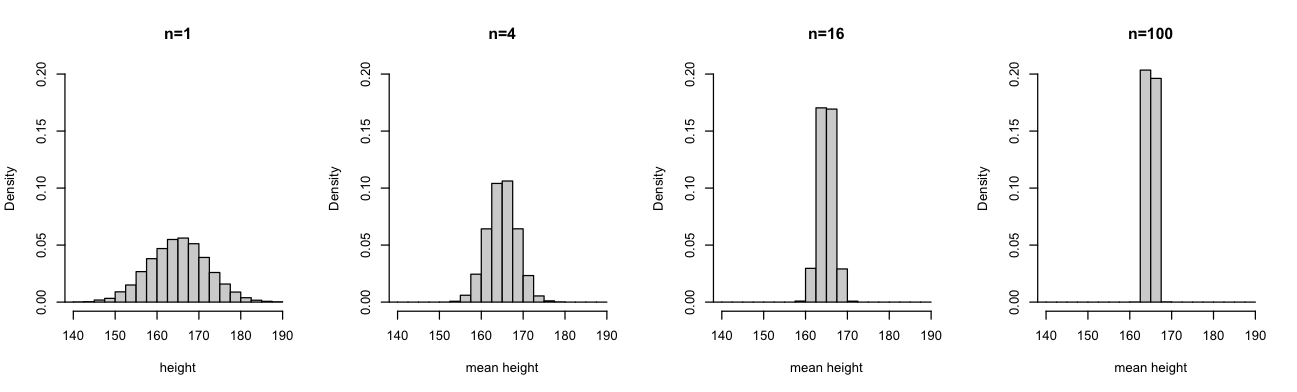
\includegraphics[width=\textwidth]{figures/05-Sampling_distribution_CLT/sampling_mean.png}
        \caption{身高平均值的抽樣分布}
        \label{fig:sampling_mean}
    \end{figure}

    \medskip

    現在我們除了抽樣之外，想做更進一步的計算：假設我們抽樣了 4 名學生並測量身高後，計算了身高的樣本平均值。此時我們有 4 個身高，但不能將它們都記為 $X$，否則就隱含了這 4 個身高都相等。為了方便區分，我們可以用 $X_1, X_2, X_3, X_4$ 來代表這 4 個身高對應的隨機變數。這 4 個隨機變數都服從 $N(165, 7 ^2)$ 的分布，而且互相獨立，所以我們可以寫作
    \smallskip
    \[X_1 \sim \NN(165, 7^2)\;\; ; \;\;X_2 \sim \NN(165, 7^2)\;\; ;X_3 \sim \NN(165, 7^2)\;\; ;X_4 \sim \NN(165, 7^2)\;\;\]
    \[X_1,X_2,X_3,X_4\text{ 相互獨立 (mutually independent)}\]
    \smallskip
    這種分布相同又相互獨立的情境在隨機抽樣中很常見，統計中給它一個專有名詞：\textit{獨立同分布} (independent and identically distributed)，簡寫為 iid。因此，我們也可以寫為
    \smallskip
    \[X_1, X_2, X_3, X_4 \overset{\text{iid}}{\sim} \NN(165, 7^2)\]
    \smallskip
    此時如果我們計算身高的平均值並令其為隨機變數 $\bar{X}$，則 $\bar{X}$ 可以寫成：
    \smallskip
    \[\bar{X} = \frac{X_1+X_2+X_3+X_4}{4}\]
    \smallskip
    可以看到 $\bar{X}$ 是由樣本 $X_1,X_2,X_3,X_4$ 計算而得的隨機變數。這種不含未知參數、由樣本計算出的隨機變數被通稱為\textit{統計量} (statistic)。由於統計量是由具有隨機的樣本計算出來的，它本身也會具有隨機性，也就是背後有一個分布。這個分布被稱為統計量的\textit{抽樣分布}（sampling distribution）。之所以被稱為抽樣分布，是因為每次抽樣得到的樣本都不同，進而計算出的統計量觀察值也會不同，而此分布目的即為描述因抽樣帶來的隨機性。

    \medskip
    
    類似前面我們所說，我們抽取 4 位學生並算出平均身高時，相當於從 $\bar{X}$ 的抽樣分布抽取一個數字。換言之，如果我們重複地「抽取 4 位學生並計算平均身高」，所得平均身高的分布即為 $\bar{X}$ 的抽樣分布，如圖\ref{fig:sampling_mean}的左二直方圖。可以看到，\textbf{統計量的抽樣分布和樣本的機率分布是完全不一樣的}，讀者一定要避免混淆。另外，如果我們不是抽取 4 位，而是抽取 16 位或 100 位學生來計算平均身高，則平均身高的抽樣分布如圖\ref{fig:sampling_mean}的右邊二個直方圖。可以看到，雖然都是平均值，但是抽取 4 位、16 位和 100 位學生計算出之平均值抽樣分布都不一樣，因此樣本數也會影響統計量的抽樣分布。

    \medskip
    
    注意到統計量的定義僅為「樣本計算出的隨機變數」，而計算的方法並不限於取樣本平均。因此，我們也可以建構其他統計量的抽樣分布：如果我們抽取 4 位、16 位或 100 位學生來計算身高樣本變異數，其抽樣分布則如圖\ref{fig:sampling_var}。可以看到這些抽樣分布均為右偏分布，和平均值的抽樣分布非常不同。總結來說，\textbf{統計量的種類和樣本數均可能影響抽樣分布的型態}。

    \begin{figure}[htbp]
        \centering
        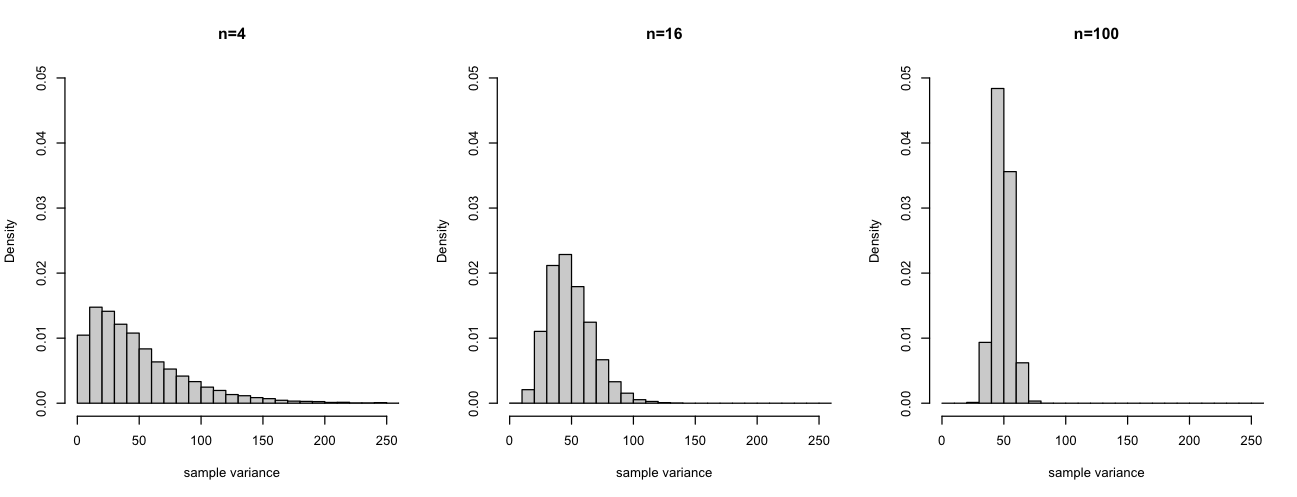
\includegraphics[width=\textwidth]{figures/05-Sampling_distribution_CLT/sampling_var.png}
        \caption{身高樣本變異數的抽樣分布}
        \label{fig:sampling_var}
    \end{figure}

    抽樣分布作為一個機率分布，也是可以計算期望值、變異數和標準差。其中統計量抽樣分布的標準差又被稱為統計量的\textit{標準誤} (standard error)。當統計量是用來估計母體參數時（例如樣本平均估計母體平均、樣本變異數估計母體變異數），統計量又被稱為\textit{估計量}（estimator），其觀察值則被稱為\textit{估計值} (estimate)。由於估計量具有變異性，估計值恰好等於母體參數的機會很低，但是我們可以藉由估計量的抽樣分布來考察估計值的表現。其中，估計量的期望值和標準誤是最直覺且重要的兩個評估點。

    \medskip
    
    如果估計量抽樣分布的期望值等於母體參數，代表估計值的取值會以母體參數為中心，我們就能比較信任這個估計量。這種估計量被稱為\textit{不偏估計量} (unbiased estimator)。例如在圖\ref{fig:sampling_mean}的左二圖中，如果我們用「四個學生的平均身高」作為清華大學生平均身高的估計量，可以看到這個估計量的抽樣分布平均值是 165，和母體平均相同，因此該估計量是不偏估計量。用符號來說，如果要估計的母體參數為 $\theta$，而我們提出的估計量是 $\hat{\theta}$，則 $\EE(\hat{\theta}) = \theta$ 時，$\hat{\theta}$ 為 $\theta$ 的不偏估計量。我們先前提到的樣本平均值、樣本變異數都是母體平均值、母體變異數的不偏估計量。

    \medskip

    估計量的標準誤代表了估計量取值的分散程度。當我們只知道估計量為不偏時，雖然估計值雖然以母體參數為中心取值，但距離母體參數的遠近則不得而知。例如圖\ref{fig:sampling_mean}中間的兩個圖中，「抽樣 4 位學生取身高平均」和「抽樣 16 位學生取身高平均」都是清華大學生身高平均值的不偏估計量，但是前者較可能出現 175, 155 這種偏離較多的估計值，後者則大多分布在 160 到 170 之間。因此，估計量的標準誤對於其估計精確程度也有影響。一般而言，我們希望估計量能夠不偏，又有很小的標準誤，這樣估計值就會非常接近母體參數。

    \medskip

    為了強化對母體分布、抽樣分布以及估計量不偏性的概念了解，讓我們同樣以抽樣清華大學學生並測量身高的例子，來思考以下的問題：

    \pagebreak

    \begin{custom}{動動腦}
        假設我們隨機找一位學生並將其身高記為 $X_1$（以公分為單位），$X_1$ 是不是一個統計量？如果我們用 $X_1$ 來估計清華大學生的平均身高，那麼該估計量是否為不偏估計量？
    \end{custom}

    \answerbox{150pt}

    \bigskip

    \begin{custom}{動動腦}
        假設我們抽樣 4 個人，並令 4 個人中最矮的人的身高為 $X_{(1)}$（以公分為單位）。請問 $X_{(1)}$ 是否為統計量？如何用重複抽樣的方式來畫出 $X_{(1)}$ 的抽樣分布？如果拿 $X_{(1)}$ 來估計清華大學生的平均身高，你覺得 $X_{(1)}$ 是否為不偏估計量？
    \end{custom}

    \answerbox{180pt}

    \bigskip

    \begin{custom}{動動腦}
        假設我們抽樣 100 人並算出身高樣本變異數 A，然後再抽樣 250 人並算出身高樣本變異數 B。這兩個樣本變異數平均而言的大小關係應該是差不多、A>B、或 A<B？
    \end{custom}

    \answerbox{200pt}
    
\section{樣本平均的抽樣分布}

    在各種統計量中，最常用的統計量就是樣本平均。因此，我們這裡針對樣本平均的統計性質作特別探討。假設我們從一個平均值為 $\mu$、變異數為 $\sigma^2$ 的母體抽出樣本數為 $n$ 的一組獨立樣本，得到的觀察值分別記為 $X_1, X_2, ..., X_n$。此時 $X_1, X_2, ..., X_n$ 為獨立同分布，期望值均為 $\mu$，變異數均為 $\sigma^2$。樣本平均可寫為
    \smallskip
    \[\bar{X} = \frac{X_1 + X_2 + ... + X_n}{n} = \frac{1}{n}\sum_{i=1}^n X_i\]
    \smallskip
    我們之前有學到隨機變數經過線性轉換後期望值和變異數的變化。我們來用這些先備知識來計算樣本平均的期望值。
    \smallskip
    \begin{align*}
        \EE(\bar{X}) &= \EE\Big(\frac{X_1 + X_2 + ... + X_n}{n}\Big)&\\
        &= \frac{1}{n}\EE(X_1 + X_2 + ... + X_n)&\text{（縮放的期望值等於期望值縮放）}\\
        &= \frac{1}{n}[\EE(X_1) + \EE(X_2) + ... + \EE(X_n)]&\text{（相加的期望值等於期望值相加）}\\
        &= \frac{1}{n}[\mu + \mu + ... + \mu]&\text{（}X_i\text{獨立同分布，期望值為}\mu\text{）}\\
        &= \frac{1}{n}[n\mu] = \mu&\\
    \intertext{因此，\textbf{樣本平均是母體平均的不偏估計量}。接下來我們來計算樣本平均的變異數。}
        var(\bar{X}) &= var\Big(\frac{X_1 + X_2 + ... + X_n}{n}\Big)&\\
        &= \frac{1}{n^2}var(X_1 + X_2 + ... + X_n)&\text{（縮放的變異數等於變異數縮放平方倍）}\\
        &= \frac{1}{n}[var(X_1) + var(X_2) + ... + var(X_n)]&\text{（獨立隨機變數相加的變異數等於變異數相加）}\\
        &= \frac{1}{n}[\sigma^2 + \sigma^2 + ... + \sigma^2]&\text{（}X_i\text{獨立同分布，變異數為}\sigma^2\text{）}\\
        &= \frac{1}{n}[n\sigma^2] = \frac{\sigma^2}{n}&
    \end{align*}
    \smallskip
    可以看到，\textbf{樣本平均的變異數是母體變異數除以樣本數}。把兩邊同時開根號後，我們得到
    \smallskip
    \[sd(\bar{X}) = \frac{\sigma}{\sqrt{n}}\]
    \smallskip
    因此，\textbf{樣本平均的標準誤是母體標準差除以根號樣本數}。因為樣本平均的標準誤太常用了，統計上給它一個專有名詞\textit{平均值標準誤} (standard error of the mean, SEM)。上述結果顯示，隨著樣本數增多，樣本平均對於母體平均的估計越來越精準，而且標準誤跟樣本數開根號呈反比。更進一步來說，當樣本數趨近於無窮大，平均值標準誤將會無限靠近零，也就是樣本平均會無限靠近母體平均。這個現象就是著名的\textit{大數法則} (Law of Large Numbers)：只要樣本是獨立同分布，隨著樣本數增至無窮大，樣本平均終究會收斂至母體平均。

    \medskip

    注意到這裡我們在描述母體時，並沒有說它是什麼分布，而只說了它的平均值為 $\mu$、變異數為 $\sigma^2$。因此，母體分布是連續型或離散型、左偏右偏或對稱並不影響我們的結論！例如於圖\ref{fig:mean_dist_bern}中，我們假設母體為機率參數 0.64 的白努利分布，機率質量函數的型態如左上角。其平均值為 $0.64$，標準差為 $\sqrt{0.64*0.36} = 0.48$。右上、左下、右下分別是樣本數為 4、25、100 的樣本平均抽樣分布。其中可以看到樣本數為 4 時只有五種可能取值，因為樣本平均為四個白努利隨機變數的平均，也就是這四次白努力實驗成功次數除以 4，可能的取值就只有 0/4、1/4、2/4、3/4、4/4 這五種。圖中樣本平均抽樣分布的平均值均在 $0.6$，也就是白努利分布的平均值。標準誤則隨著樣本數增加而逐漸降低（分布逐漸變窄），且我們可以精確的算出各樣本數下的平均值標準誤。當 $n=4$ 時，標準誤應為 $\frac{0.48}{\sqrt{4}} = 0.12$、當$n=100$時，標準誤應為$\frac{0.48}{\sqrt{100}} = 0.048$。這種期望值不變，標準誤下降的現象在其他分布也同樣會出現，圖\ref{fig:mean_dist_unif}即用連續型的標準均一分布作為母體。

    \begin{figure}[htbp]
        \centering
        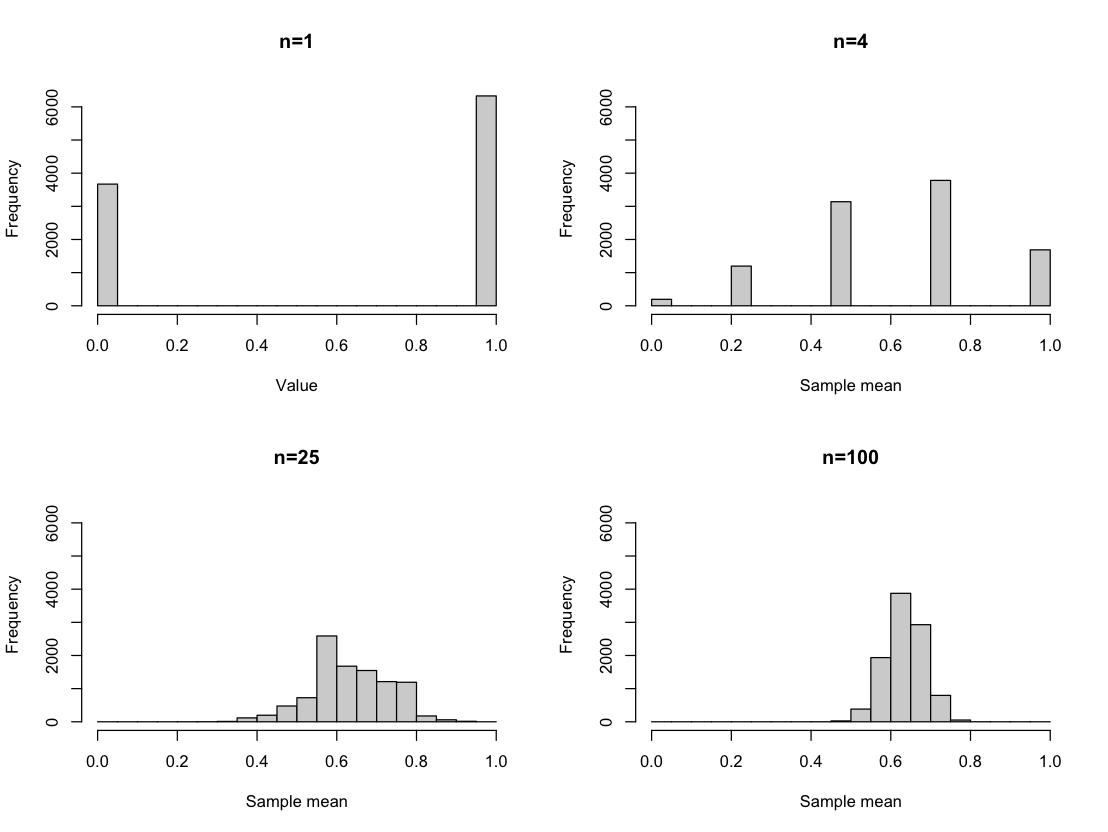
\includegraphics[width=0.9\textwidth]{figures/05-Sampling_distribution_CLT/mean_dist_bern.png}
        \caption{母體為 $Bernoulli(0.6)$ 的樣本平均抽樣分布}
        \label{fig:mean_dist_bern}
    \end{figure}

    \begin{figure}[htbp]
        \centering
        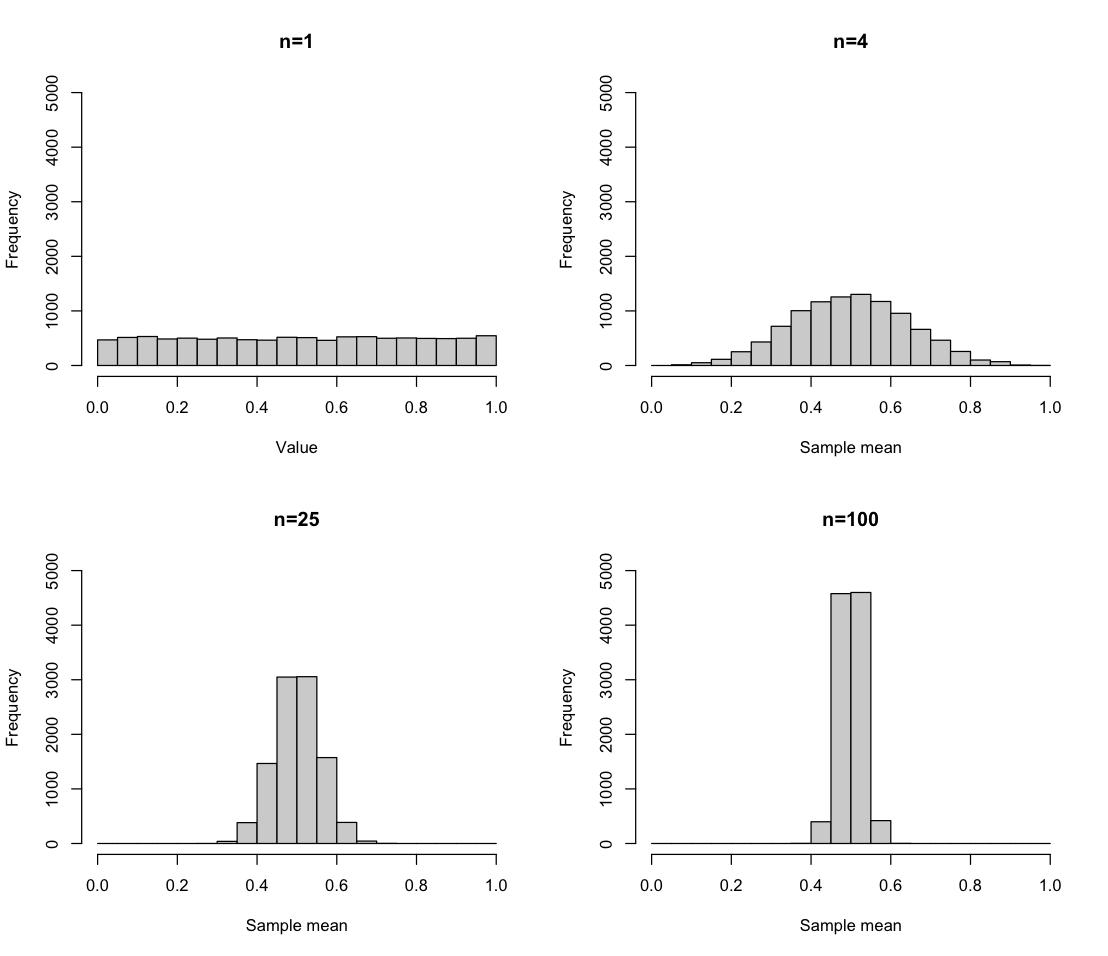
\includegraphics[width=0.8\textwidth]{figures/05-Sampling_distribution_CLT/mean_dist_unif.png}
        \caption{母體為標準均一分布的樣本平均抽樣分布}
        \label{fig:mean_dist_unif}
    \end{figure}

    從圖\ref{fig:mean_dist_bern}和\ref{fig:mean_dist_unif}可以看出，即便我們可以由母體的期望值和標準差精準計算出樣本平均抽樣分布的期望值和標準差，該抽樣分布的實際長相卻仍然取決於母體分布的型態。大多數的時候，這些平均值抽樣分布不在我們常用分布之列，但有一個特殊例外：\textbf{當母體服從常態分布時，樣本平均也會服從常態分布}。由於常態分布只有兩個參數：平均值和變異數，而我們已知樣本平均的期望值是母體平均值 $\mu$，變異數是母體變藝術除以樣本數 $\sigma^2/n$，所以我們可以直接寫出樣本平均的分布：
    \smallskip
    \[\bar{X} \sim \NN\Big(\mu, \frac{\sigma^2}{n}\Big)\]
    \smallskip
    舉例而言，如果已知 60-70 歲男性的收縮壓 (mmHg) 分布服從 $\NN(130, 10)$ 的常態分布，那麼抽樣 16 位 60-70 歲男性算出的平均收縮壓就應該服從 $\NN(130, 10/\sqrt{16} = 2.5)$。我們還能依此算出平均收縮壓介於某個區間的機率，例如該平均收縮壓介於 125 至 135 mmHg 的機率為
    \[\PP(125 \le \bar{X} \le 135) = \PP\Big(\frac{125-130}{2.5} \le \frac{\bar{X}-130}{2.5} \le \frac{125-130}{2.5}\Big) = \PP(-2 \le \ZZ \le 2) \approx 0.954\]
    
    \bigskip

    \begin{custom}{動動腦}
        假設我們從平均值為 150 、標準差為 5 的母體抽出一個樣本數為 25 的樣本，則樣本標準差應該會最接近下列哪個數值：(1) 5 (2) 1 (3) 1/5。
    \end{custom}

    \answerbox{110pt}

    \bigskip

    \begin{custom}{動動腦}
        回到清華大學生的例子。假設我們不知道清華大學生身高的分布，因此隨機抽取了三位學生來量身高，分別是 160、165、170 公分，並得到樣本平均值 165 公分以估計母體平均。請問我們是否知道該樣本平均的標準誤確切數值？若否，如何用資料來估計該樣本平均的標準誤？
    \end{custom}

    \answerbox{130pt}

    \bigskip

    \begin{custom}{動手作}
        根據一項大型世代研究，45 歲以上氣喘患者的平均急性發作率為一年 0.22 次。假設一年氣喘的發作次數可用卜瓦松分布來描述。現由 45 歲以上氣喘患者中隨機抽取 100 人並計算他們平均一年氣喘發作的次數。該平均次數的期望值和標準誤應為何？
    \end{custom}

    \answerbox{180pt}

    \bigskip

    \begin{custom}{動動腦}
        在醫學流病的應用研究中，通常會有製作一個 Table 1 來描述納入族群的特徵，例如性別比例、年齡、慢性病史比例等等。針對連續型變項例如年齡，假設樣本平均為 55 歲，樣本標準差為 10 歲，樣本數為 100 人，那麼年齡的敘述性統計應該寫成 $55 \pm 10$ （正負標準差）比較合理，還是 $55 \pm 1$ （正負標準誤）比較合理？
    \end{custom}

    \answerbox{180pt}

\section{中央極限定理}
    我們前面探討平均值抽樣分布的性質時，關注了它的期望值和標準差（即平均值標準誤），並且僅知道當母體為常態分布時，樣本平均亦服從常態分布。然而，當母體非常態分布時，我們對於樣本平均的抽樣分布形狀沒有太多概念。觀察圖\ref{fig:mean_dist_bern}和\ref{fig:mean_dist_unif}可以看到，當樣本數比較少(n = 4, 25)的時候，平均值抽樣分布的型態較為取決於母體分布。例如母體為左偏的白努利分布時，平均值抽樣分布還是有點離散，而且大致上是左偏。不過當樣本數變大時(n = 100)，兩個母體分布下的樣本平均抽樣分布都呈現大致對稱的鐘型。這個鐘型分布不是別的分布：正是常態分布！\textbf{不論母體分布為何}，只要樣本數不斷增大，樣本平均抽樣分布都會趨近於常態分布。由於常態分布只有兩個參數：平均值與變異數，而我們在前一節已經導出樣本平均抽樣分布的平均值（母體平均）與變異數（母體變異數除以樣本數），所以這個趨近的常態分布就完全已知了。以上就是統計中最重要的\textit{中央極限定理} (Central Limit Theorem, CLT)：

    \begin{theorem*}{（中央極限定理）}
        若 $X_1, X_2, ... X_n$ 為獨立同分布、平均值為 $\mu$、變異數為 $\sigma^2$ 的隨機變數，令樣本平均 $\bar{X} = \frac{1}{n}\sum_{i=1}^n X_i$，則
        \[\frac{\bar{X}-\mu}{\sigma/\sqrt{n}} \leadsto \NN(0,1)\]
        或
        \[\bar{X} \leadsto \NN\Big(\mu,\frac{\sigma^2}{n}\Big)\]
    \end{theorem*}
    \noindent（註：這裡我們用$\leadsto$來代表分布在樣本數大時近似。按統計的定義 $\bar{X} \leadsto \NN\big(\mu,\frac{\sigma^2}{n}\big)$的寫法其實不太嚴謹，但這裡我們只強調概念）

    \medskip
    
    中央極限定理精要就是\textbf{任何母體的樣本平均抽樣分布，在樣本「夠大」的情況下，會趨近於常態分布}。至於怎樣才叫「夠大」，理論上要視母體分布的偏斜和厚尾程度而定，但一般會認為樣本數大於 30 就足夠讓我們用常態分布來\textbf{近似}平均值抽樣分布。

    \medskip
    
    利用中央極限定理，只要統計量是由樣本平均算出的，我們就可以寫出它在樣本數夠大時的近似分布，進而計算出其數值在指定區間的機率。例如，如果我們做一份 $n$ 人的民調，調查對於某議案的支持度，那麼每個民調受訪者是否支持（將支持記為 $1$、不支持記為 $0$）其實都服從一個機率參數為 $p$ 的白努利分布，其中 $p$ 為全民對該議案的支持度。民調最後顯示支持度 $\hat{p}$ 是將總支持人數除以總受訪人數，即為這些白努利分布隨機變數的平均值。根據中央極限定理，因為白努利分布的期望值為 $p$、變異數為 $p(1-p)$：
    \smallskip
    \[\hat{p} \leadsto \NN\Big(p, \frac{p(1-p)}{n}\Big)\]
    \smallskip
    因此，一個實際支持率為 $60\%$ 的議案，若做一份 $600$ 人的民調，其民調支持率 $\hat{p}$ 應趨近服從 $\NN(0.6, \frac{0.6 \cdot 0.4}{600} = 0.0004)$。根據這個近似抽樣分布，民調支持率低於 $55\%$ 的機率可以如下計算：
    \smallskip
    \[\PP(\hat{p} \le 0.55) = \PP\Big(\frac{\hat{p}-0.6}{\sqrt{0.0004}} \le \frac{0.55-0.6}{\sqrt{0.0004}}\Big) \approx \PP(\ZZ \le -2.5) \approx 0.00621\]
    \smallskip
    注意到如果我們把民調支持率乘上樣本數，就會得到支持人數。根據平均值與變異數的性質，支持人數 $Y$ 的近似抽樣分布可寫為
    \smallskip
    \[Y = n\hat{p} \leadsto \NN(np, np(1-p))\]
    \smallskip
    根據二項式分布的定義，支持人數的精確分布應該是次數參數為 $n$、機率參數為 $p$ 的二項式分布。這意味著二項式分布在次數參數 $n$ 足夠大的時候，可以用平均值與變異數相仿的常態分布來近似，也就是
    \smallskip
    \[\text{Binomial}(n, p) \leadsto \NN(np, np(1-p))\]
    \smallskip
    至於怎樣叫作「足夠大」，一般認為 $np$ 和 $n(1-p)$ 均大於 $10$ 的時候近似效果就很好。同樣地，由於卜瓦松分布是二項式分布在 $np=\lambda$ 且 $n$ 趨近無限大時的分布，所以當 $\lambda > 10$ 時，我們也可以做以下的近似
    \smallskip
        \[\text{Poisson}(\lambda) \leadsto \NN(\lambda, \lambda)\]

    使用常態分布近似二項分布或卜瓦松分布時，為了讓近似更加準確，經常會引進\textit{連續性校正} (continuity correction)，也就是把 $\PP(X = x)$ 的機率用常態分布中的 $\PP(x-0.5 \le X \le x + 0.5)$ 來近似。舉例來說，如果 $X \sim Poisson(36)$，且我們想計算 $32 \le X \le 37$ 的機率。因為速率參數已經大於 10，我們可以試著用 $\NN(36, 36)$ 來近似 $X$ 的分布。此時 $32 \le X \le 37$ 的機率，套用連續性校正後變成求 $31.5 \le X \le 37.5$ 的機率，因此計算如下
    \smallskip
    \begin{align*}
        \PP(31.5 \le X \le 37.5) &= \PP\Big(\frac{31.5-36}{\sqrt{36}} \le \frac{X-36}{\sqrt{36}} \le \frac{37.5-36}{\sqrt{36}}\Big)\\
        &\approx \PP(-0.75 \le \ZZ \le 0.25)\\
        &\approx (1-0.401)-0.227\\
        &= 0.372
    \end{align*}
    \smallskip
    如果實際用卜瓦松分布的機率質量函數計算 $\PP(32 \le X \le 37) = \sum_{j=32}^{37} \frac{36^j e^{-36}}{j!} \approx 0.378$，可見近似的效果還不錯。
    
    \medskip
    
    除了用來作統計量的分布近似外，中央極限定理在推論統計的其他工具中扮演了舉足輕重的角色。讀者必須熟知此定理的概念以及適用前提，我們會在未來的課程中反覆使用這個重要的定理。

    \bigskip

    \begin{custom}{動手作}
        某總統大選民調預計調查 $1,110$ 位公民之投票意向為候選人甲或候選人乙。假設所有公民均會在兩位候選人中挑選一位，當兩位候選人之實際支持率相同時，調查結果顯示候選人甲之支持率領先候選人乙 $6\%$ 之機率為何？
    \end{custom}

    \answerbox{230pt}

    \bigskip
    
    \begin{custom}{動手作}
        根據研究，服用降低血脂的 statin 類藥物出現嚴重肌病變的機率約為五千分之一。台灣的糖尿病與高血壓患者約有八萬五千人正在接受 statin 類藥物治療，試計算出現嚴重肌病變人數在 25 人以上的機率。
    \end{custom}
    
    \answerbox{230pt}

    \bigskip
    
    \begin{takehome}
        \item 統計量是由樣本計算、不含任何參數的量。統計量的分布稱為其抽樣分布。
        \item 用於估計參數的統計量稱為估計量。估計量的標準差通常又稱為標準誤。
        \item 若一個估計量的期望值等於其所估計的參數，則稱該估計量為不偏估計量。
        \item 如果兩個估計量均為不偏估計量，則我們傾向標準誤較小的估計量，因為其不確定性較低。
        \item 當樣本觀測值獨立且同分布時：
        \begin{enumerate}
            \item 樣本平均值的期望值等於母體平均數。
            \item 樣本平均值的標準誤等於母體標準差除以樣本數的平方根。
            \item 大數法則：隨著樣本數增加，樣本平均值將愈來愈接近母體平均數。
            \item 當母體為常態分布時，樣本平均值的抽樣分布為準確的常態分布。
            \item 中央極限定理：隨著樣本數增加，樣本平均值的分布將愈來愈接近常態分布。
        \end{enumerate}
    \end{takehome}

    \bigskip

    \begin{docexam}{（107-2醫學(二)）}
        下列何者不是中央極限定理的涵義？
        
        (A) 隨機樣本平均值之統計分布接近常態分布
        
        (B) 隨機樣本平均值之統計分布接近布阿松分布 (Poisson distribution)
        
        (C) 所有可能的隨機樣本平均值之平均值等於母群體平均值
        
        (D) 標準誤取決於母群體標準差與樣本的大小
    \end{docexam}

    \pagebreak

    \begin{docexam}{（105-2醫學(一)）}
        下列對中央極限定理的描述，何者錯誤？
        
        (A) 只要樣本數夠大，無論原本母群體是否為常態分布，樣本平均值的抽樣分布會接近常態分布
        
        (B) 母群體的平均值若為 $\mu$，則樣本平均值抽樣分布的平均值為 $\mu$
        
        (C) 母群體的標準差若為 $\sigma$，則樣本平均值抽樣分布的標準差為 $\sigma/n$
        
        (D) 可透過中央極限定理將樣本平均值的抽樣分布變成標準常態分布
    \end{docexam}

    \begin{docexam}{（104-1醫學(一)）}
        下列對中央極限定理的敘述，何者錯誤？
        
        (A) 只要樣本數夠大，樣本平均數的分布就會趨近常態分布
        
        (B) 只要樣本數夠大，樣本平均數分布的期望值就會很接近母體平均數
        
        (C) 只要樣本數超過 1，樣本平均數分布的標準差都會小於母體標準差
        
        (D) 母體分布只有在常態分布時，樣本數夠大時樣本平均數的分布才會趨近常態分布
    \end{docexam}

    \begin{docexam}{（103-2醫學(一)）}
        一個等距尺度之臨床變數為雙峰分布，以大樣本經過多次重複抽樣之後，其樣本平均數的抽樣分布為一個常態分布。此現象反應下列何種定理？
        
        (A) 中央極限定理
        
        (B) 貝氏定理
        
        (C) 機率總和定理
        
        (D) 二項式定理
    \end{docexam}

    \begin{docexam}{（103-1醫學(一)）}
        當樣本統計量與母群體母數之差的平均值為0，亦即統計量的期望值等於母數。此統計量具有下列何種統計學特性？
        
        (A) 有效性
        
        (B) 一致性
        
        (C) 充分性
        
        (D) 不偏性
    \end{docexam}

    \begin{docexam}{（102-2醫學(一)）}
        下列對中央極限定理的敘述何者錯誤？
        
        (A) 樣本平均數之抽樣分布的標準差又稱標準誤，其值等於樣本標準差除以樣本數
        
        (B) 樣本平均數之抽樣分布的平均值等於母體平均值
        
        (C) 如果母群體為常態分布，即便樣本數不大，樣本平均數之抽樣分布也會接近常態分布
        
        (D) 如果樣本數夠大，則樣本平均數之抽樣分布定會接近常態分布
    \end{docexam}